% Digital Logic Report Template
% Created: 2020-01-10, John Miller

%==========================================================
%=========== Document Setup  ==============================

% Formatting defined by class file
\documentclass[11pt]{article}

% ---- Document formatting ----
\usepackage[margin=1in]{geometry}	% Narrower margins
\usepackage{booktabs}				% Nice formatting of tables
\usepackage{graphicx}				% Ability to include graphics

%\setlength\parindent{0pt}	% Do not indent first line of paragraphs 
\usepackage[parfill]{parskip}		% Line space b/w paragraphs
%	parfill option prevents last line of pgrph from being fully justified

% Parskip package adds too much space around titles, fix with this
\RequirePackage{titlesec}
\titlespacing\section{0pt}{8pt plus 4pt minus 2pt}{3pt plus 2pt minus 2pt}
\titlespacing\subsection{0pt}{4pt plus 4pt minus 2pt}{-2pt plus 2pt minus 2pt}
\titlespacing\subsubsection{0pt}{2pt plus 4pt minus 2pt}{-6pt plus 2pt minus 2pt}

% ---- Hyperlinks ----
\usepackage[colorlinks=true,urlcolor=blue]{hyperref}	% For URL's. Automatically links internal references.

% ---- Code listings ----
\usepackage{listings} 					% Nice code layout and inclusion
\usepackage[usenames,dvipsnames]{xcolor}	% Colors (needs to be defined before using colors)

% Define custom colors for listings
\definecolor{listinggray}{gray}{0.98}		% Listings background color
\definecolor{rulegray}{gray}{0.7}			% Listings rule/frame color

% Style for Verilog
\lstdefinestyle{Verilog}{
	language=Verilog,					% Verilog
	backgroundcolor=\color{listinggray},	% light gray background
	rulecolor=\color{blue}, 			% blue frame lines
	frame=tb,							% lines above & below
	linewidth=\columnwidth, 			% set line width
	basicstyle=\small\ttfamily,	% basic font style that is used for the code	
	breaklines=true, 					% allow breaking across columns/pages
	tabsize=3,							% set tab size
	commentstyle=\color{gray},	% comments in italic 
	stringstyle=\upshape,				% strings are printed in normal font
	showspaces=false,					% don't underscore spaces
}

% How to use: \Verilog[listing_options]{file}
\newcommand{\Verilog}[2][]{%
	\lstinputlisting[style=Verilog,#1]{#2}
}




%======================================================
%=========== Body  ====================================
\begin{document}

\title{ELC 2137 Lab \#3: Adders}
\author{Xingpeng Yi and Maya Martin}

\maketitle


\section*{Summary}

To complete the Adders lab students were required to build and design logical circuits given the required outputs. In order to minimize both human and hardware error, it is imperative that students draw out each circuit with corresponding gates, LED’s, GND, Voltage, and correct current flow through each path. By doing this student’s are able to visualize the logical side of the circuits as well as catch any future mistakes that might occur throughout the lab. Once a diagram has been built, students were responsible for fulfilling a circuit with the desired outcome. By the end of the lab, students should be able to complete a functioning Full Adder, Two-Bit Adder, Half-Bit Adder on both papers and on a circuit board. 


\section*{Q\&A}

\begin{enumerate}
	\item  Which gates could we use for combining the carry bits?
	
	Based on the truth table, a OR gate needs to be use for the carry bits. Only one carry needs to be true, the out carry will be true. It is an OR gate. The frsit and second carry are not true at same time, so an XOR gate is also fine.
	
	\item Which one should we use and why?
	
	A OR gate should be used in the lab, but XOR gate is also fine. In the lab, 7486 chip is used.  The chip has four XOR gates.The carry1 and carry 2 are not true at teh same time. It is true when one of the carry is true, so using a XOR will be identical as using OR gate.
\end{enumerate}


\section*{Results}

In this section, put your simulation waveforms, results tables, pictures of hardware, and any other required items.\begin{table}[ht]\centering
	\caption{2-bit adder truth table}
	\label{tbl:example_table}
	\begin{tabular}{ccccc|ccc}
		\toprule
		Cin & A2 & A1 & B2 & B1 & Cout & S2 & S1\\
		\midrule
		0 & 0 & 0 & 0 & 0 & 0 & 0 & 0 \\
		0 & 0 & 0 & 0 & 1 & 0 & 0 & 1 \\
		0 & 0 & 1 & 0 & 1 & 0 & 1 & 0 \\
		0 & 1 & 0 & 0 & 1 & 0 & 1 & 1 \\
		0 & 1 & 0 & 1 & 0 & 1 & 0 & 0 \\
		1 & 1 & 0 & 1 & 0 & 1 & 0 & 1 \\
		1 & 1 & 1 & 1 & 1 & 1 & 1 & 1 \\
		
		\bottomrule
	\end{tabular} 
\end{table}
According to the the table above, 

\includegraphics[width=\textwidth]{"circuit demonstration page"}

\section*{Circuits}

\begin{figure}[ht]\centering
	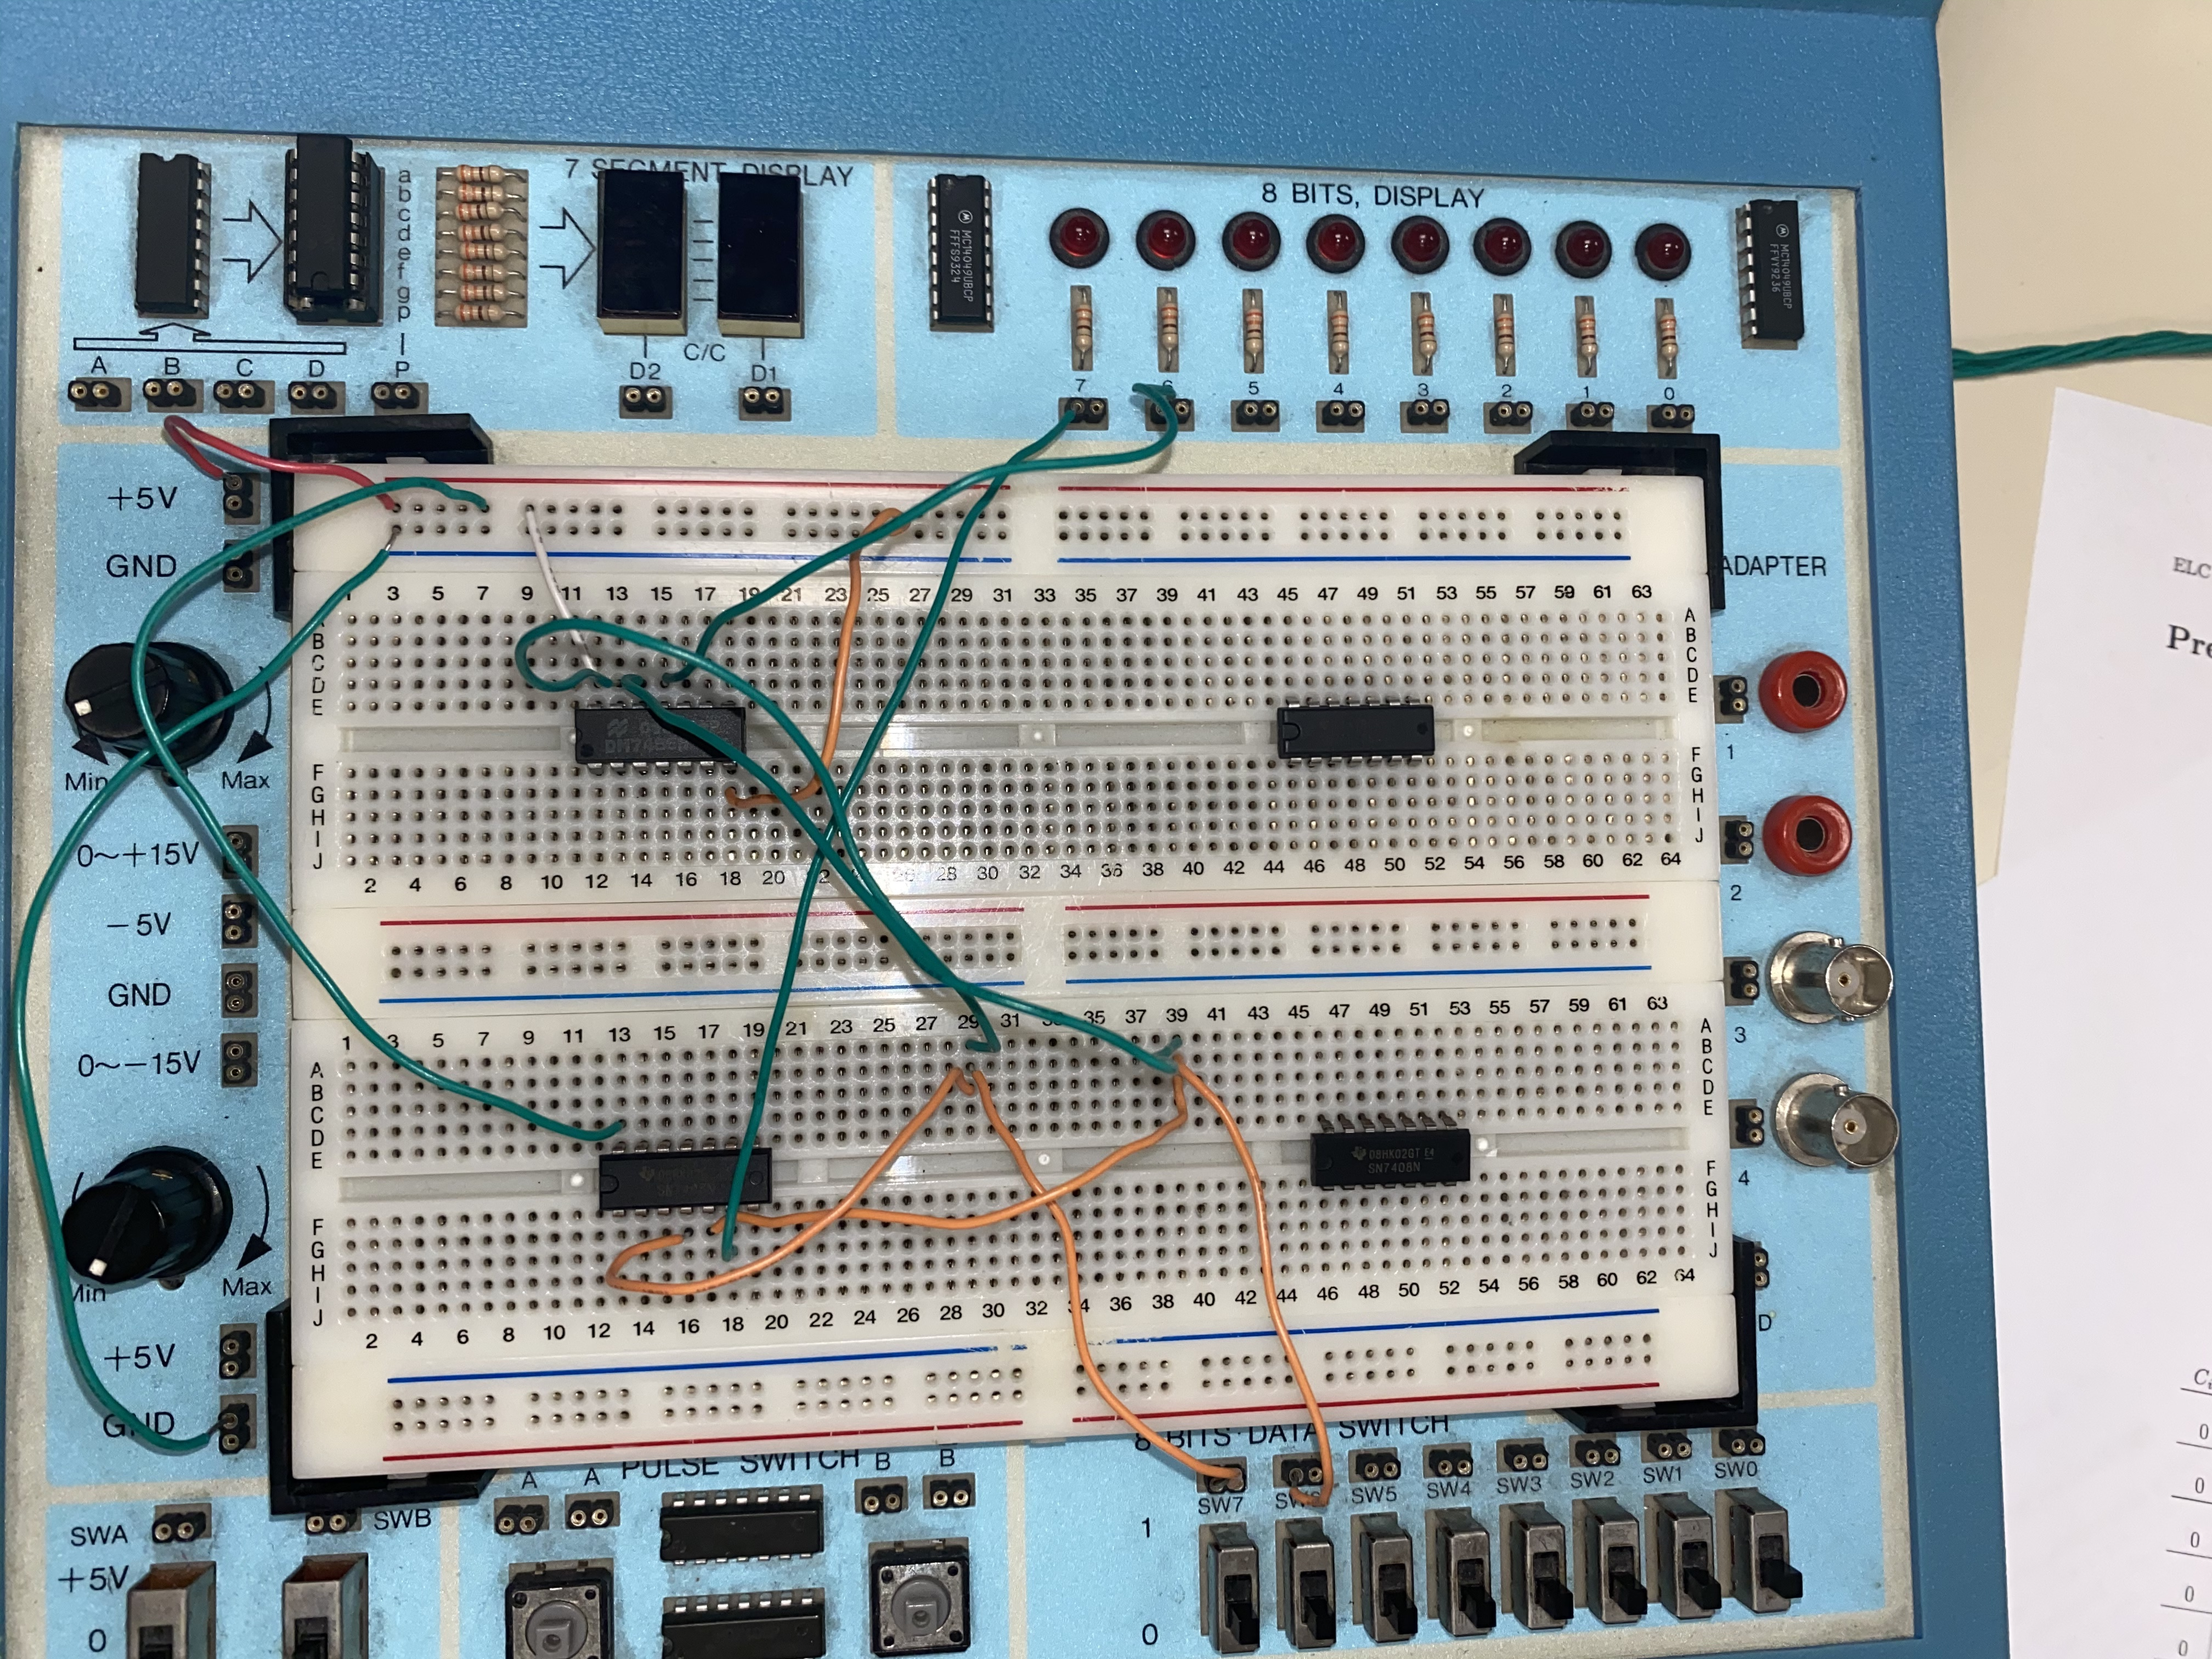
\includegraphics[width=0.5\textwidth]{halfadder}
	\caption{This is the half adder.}
	\label{fig:half adder}			% label must be after caption
\end{figure}
There is a lack of the full adder pictures, but the left half of the  2-bit adder is full adder circuit.

\begin{figure}[ht]\centering
	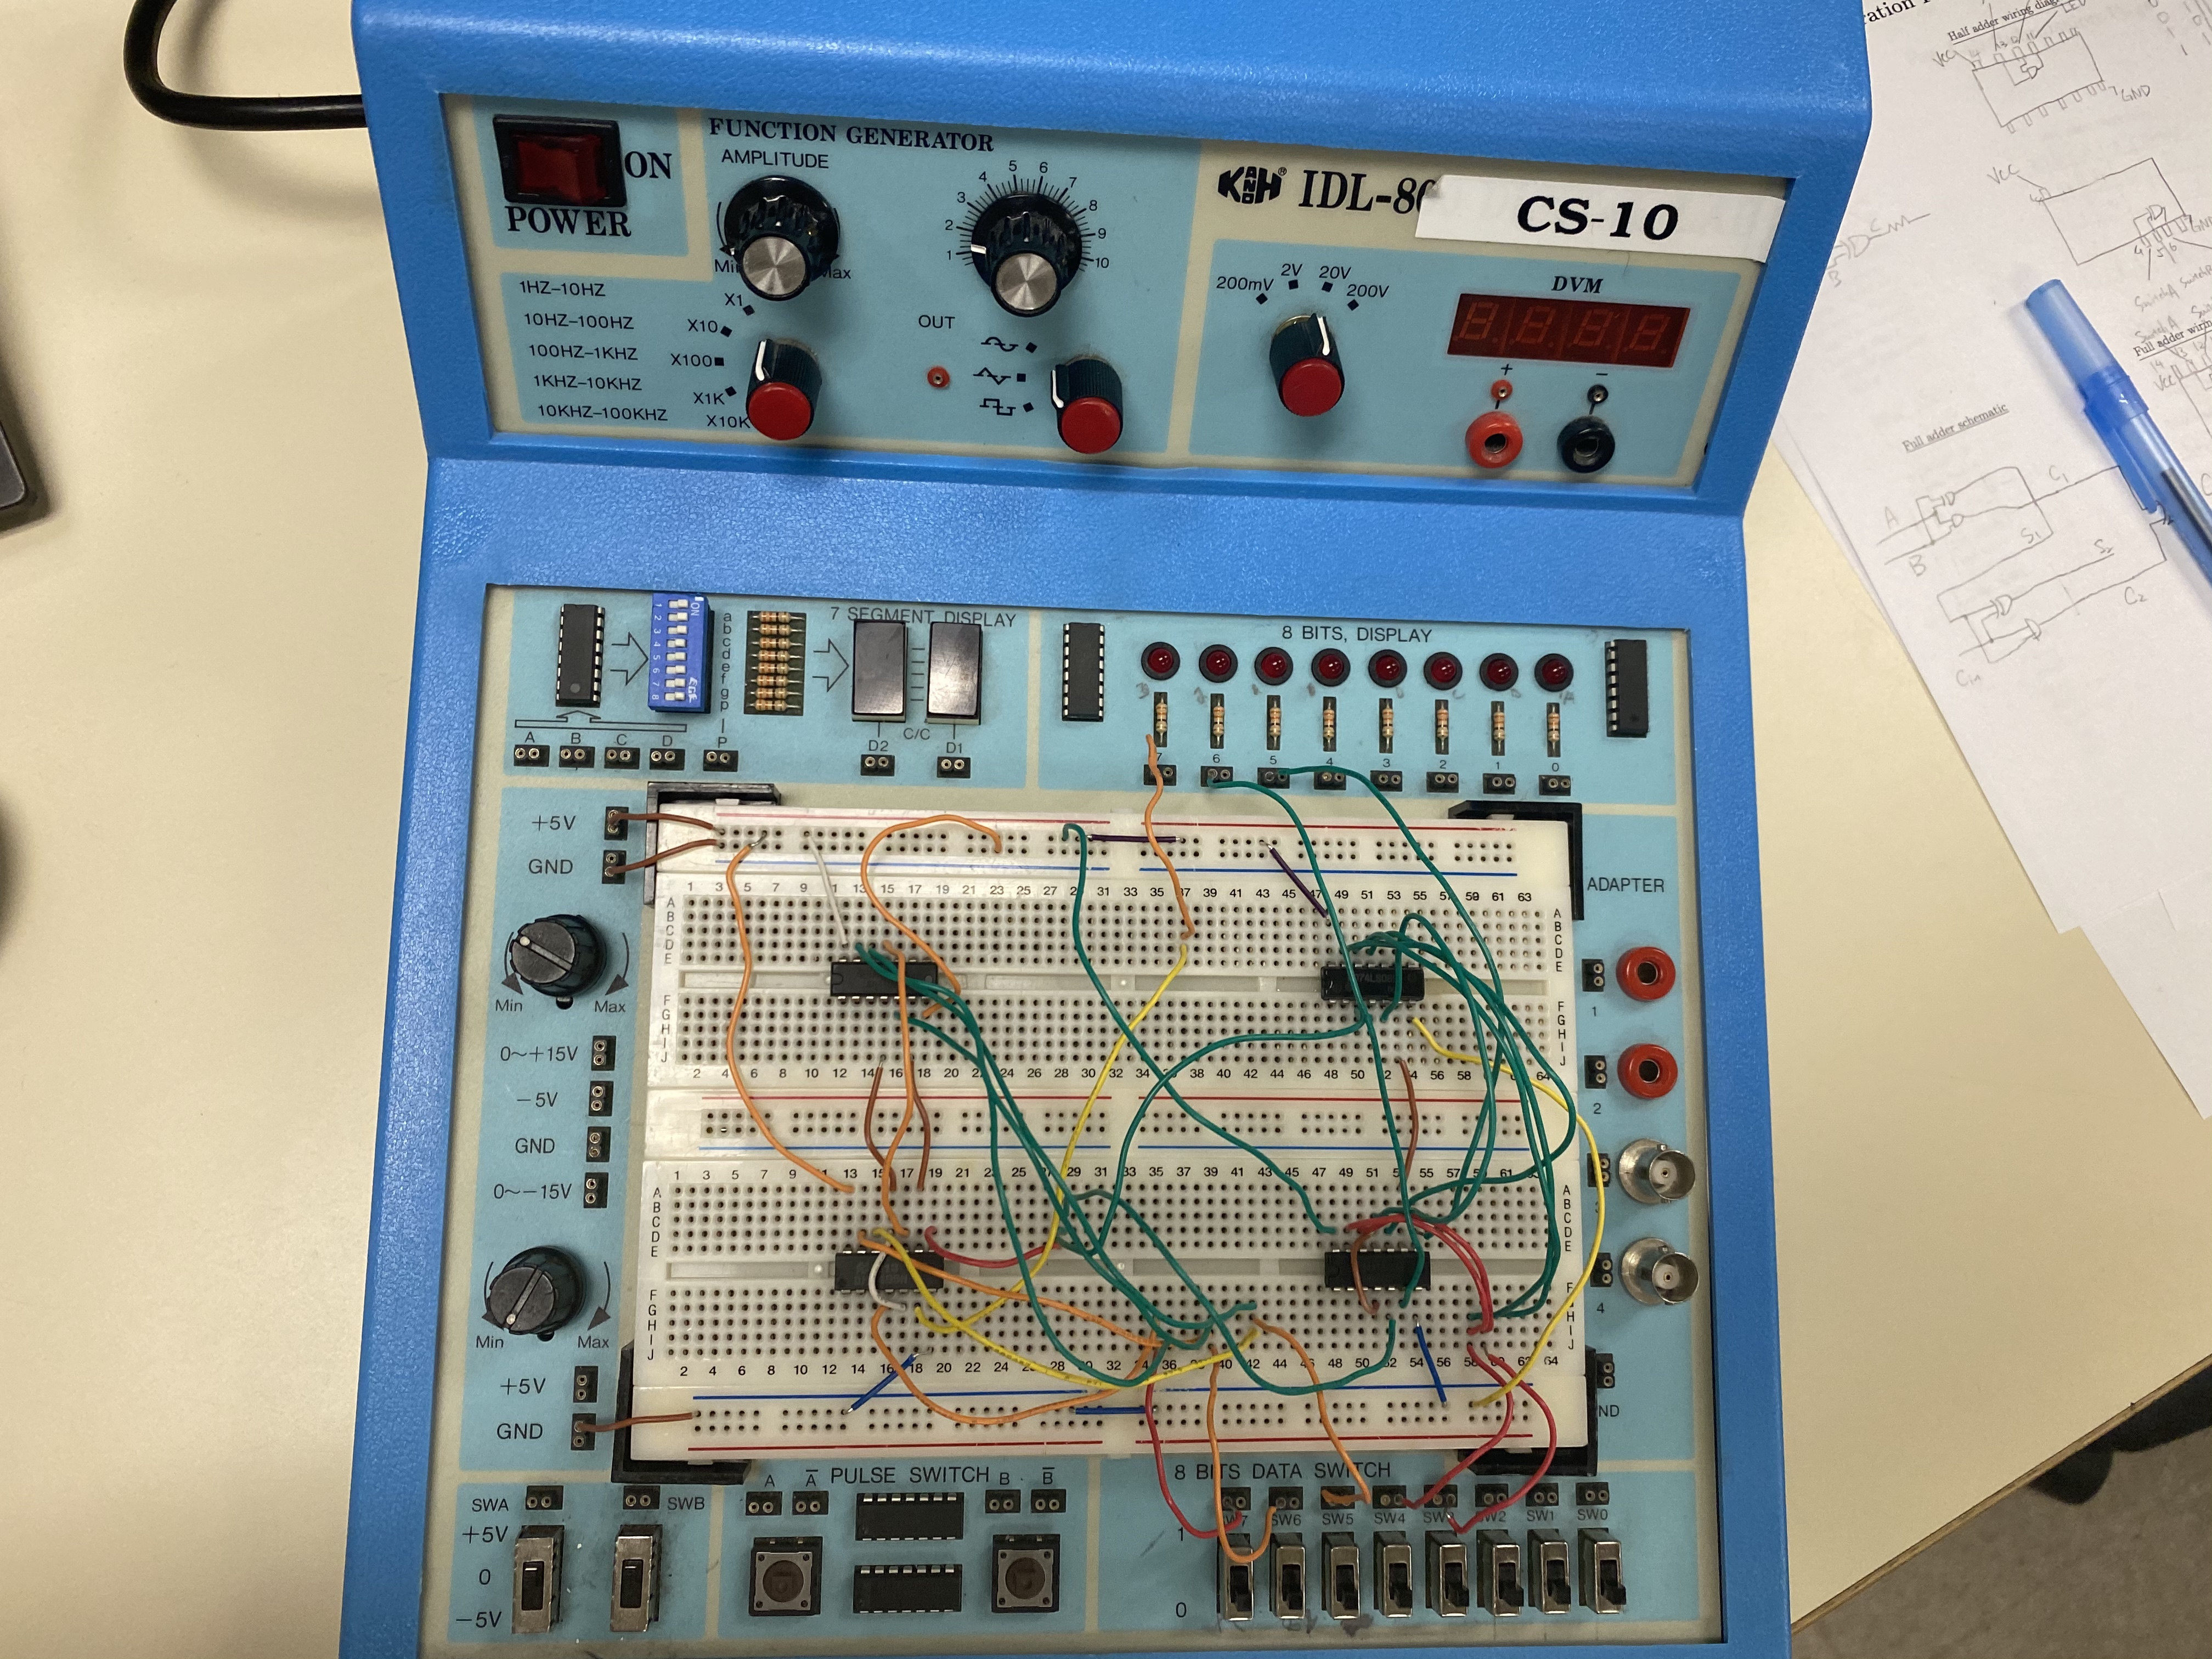
\includegraphics[width=0.5\textwidth]{2-bitadder}
	\caption{This is the 2-bit adder.}
	\label{fig:2-bit adder}			% label must be after caption
\end{figure}

\section*{Conclusion}
In half adders, the carry follows an AND gate,  the sum is a NOR gate. In the full adder, it is a combination of two half adders. The sum of  first HA is connected to the third input to another HA. The carry of  second HA and the first carry go through an OR gate and result in the out carry of the FA. The 2-bit adder is a combination of 2 FAs. The out carry of the first FA is the third input of the second FA. Sum of the first FA and the sum of second FA are connected to the LED. The out carry of the second FA is the out carry of the 2-bit adder. In this lab, the OR gates are all replaced by XOR gates. In the truth table, the two carry in the FA shows a OR gate property, but these two carry never been true at the same time. Under this circumstance, using XOR gates is identical to OR gates.
\end{document}
